\section{Results}\label{sec:results}

\begin{figure}[ht]
    \centering
    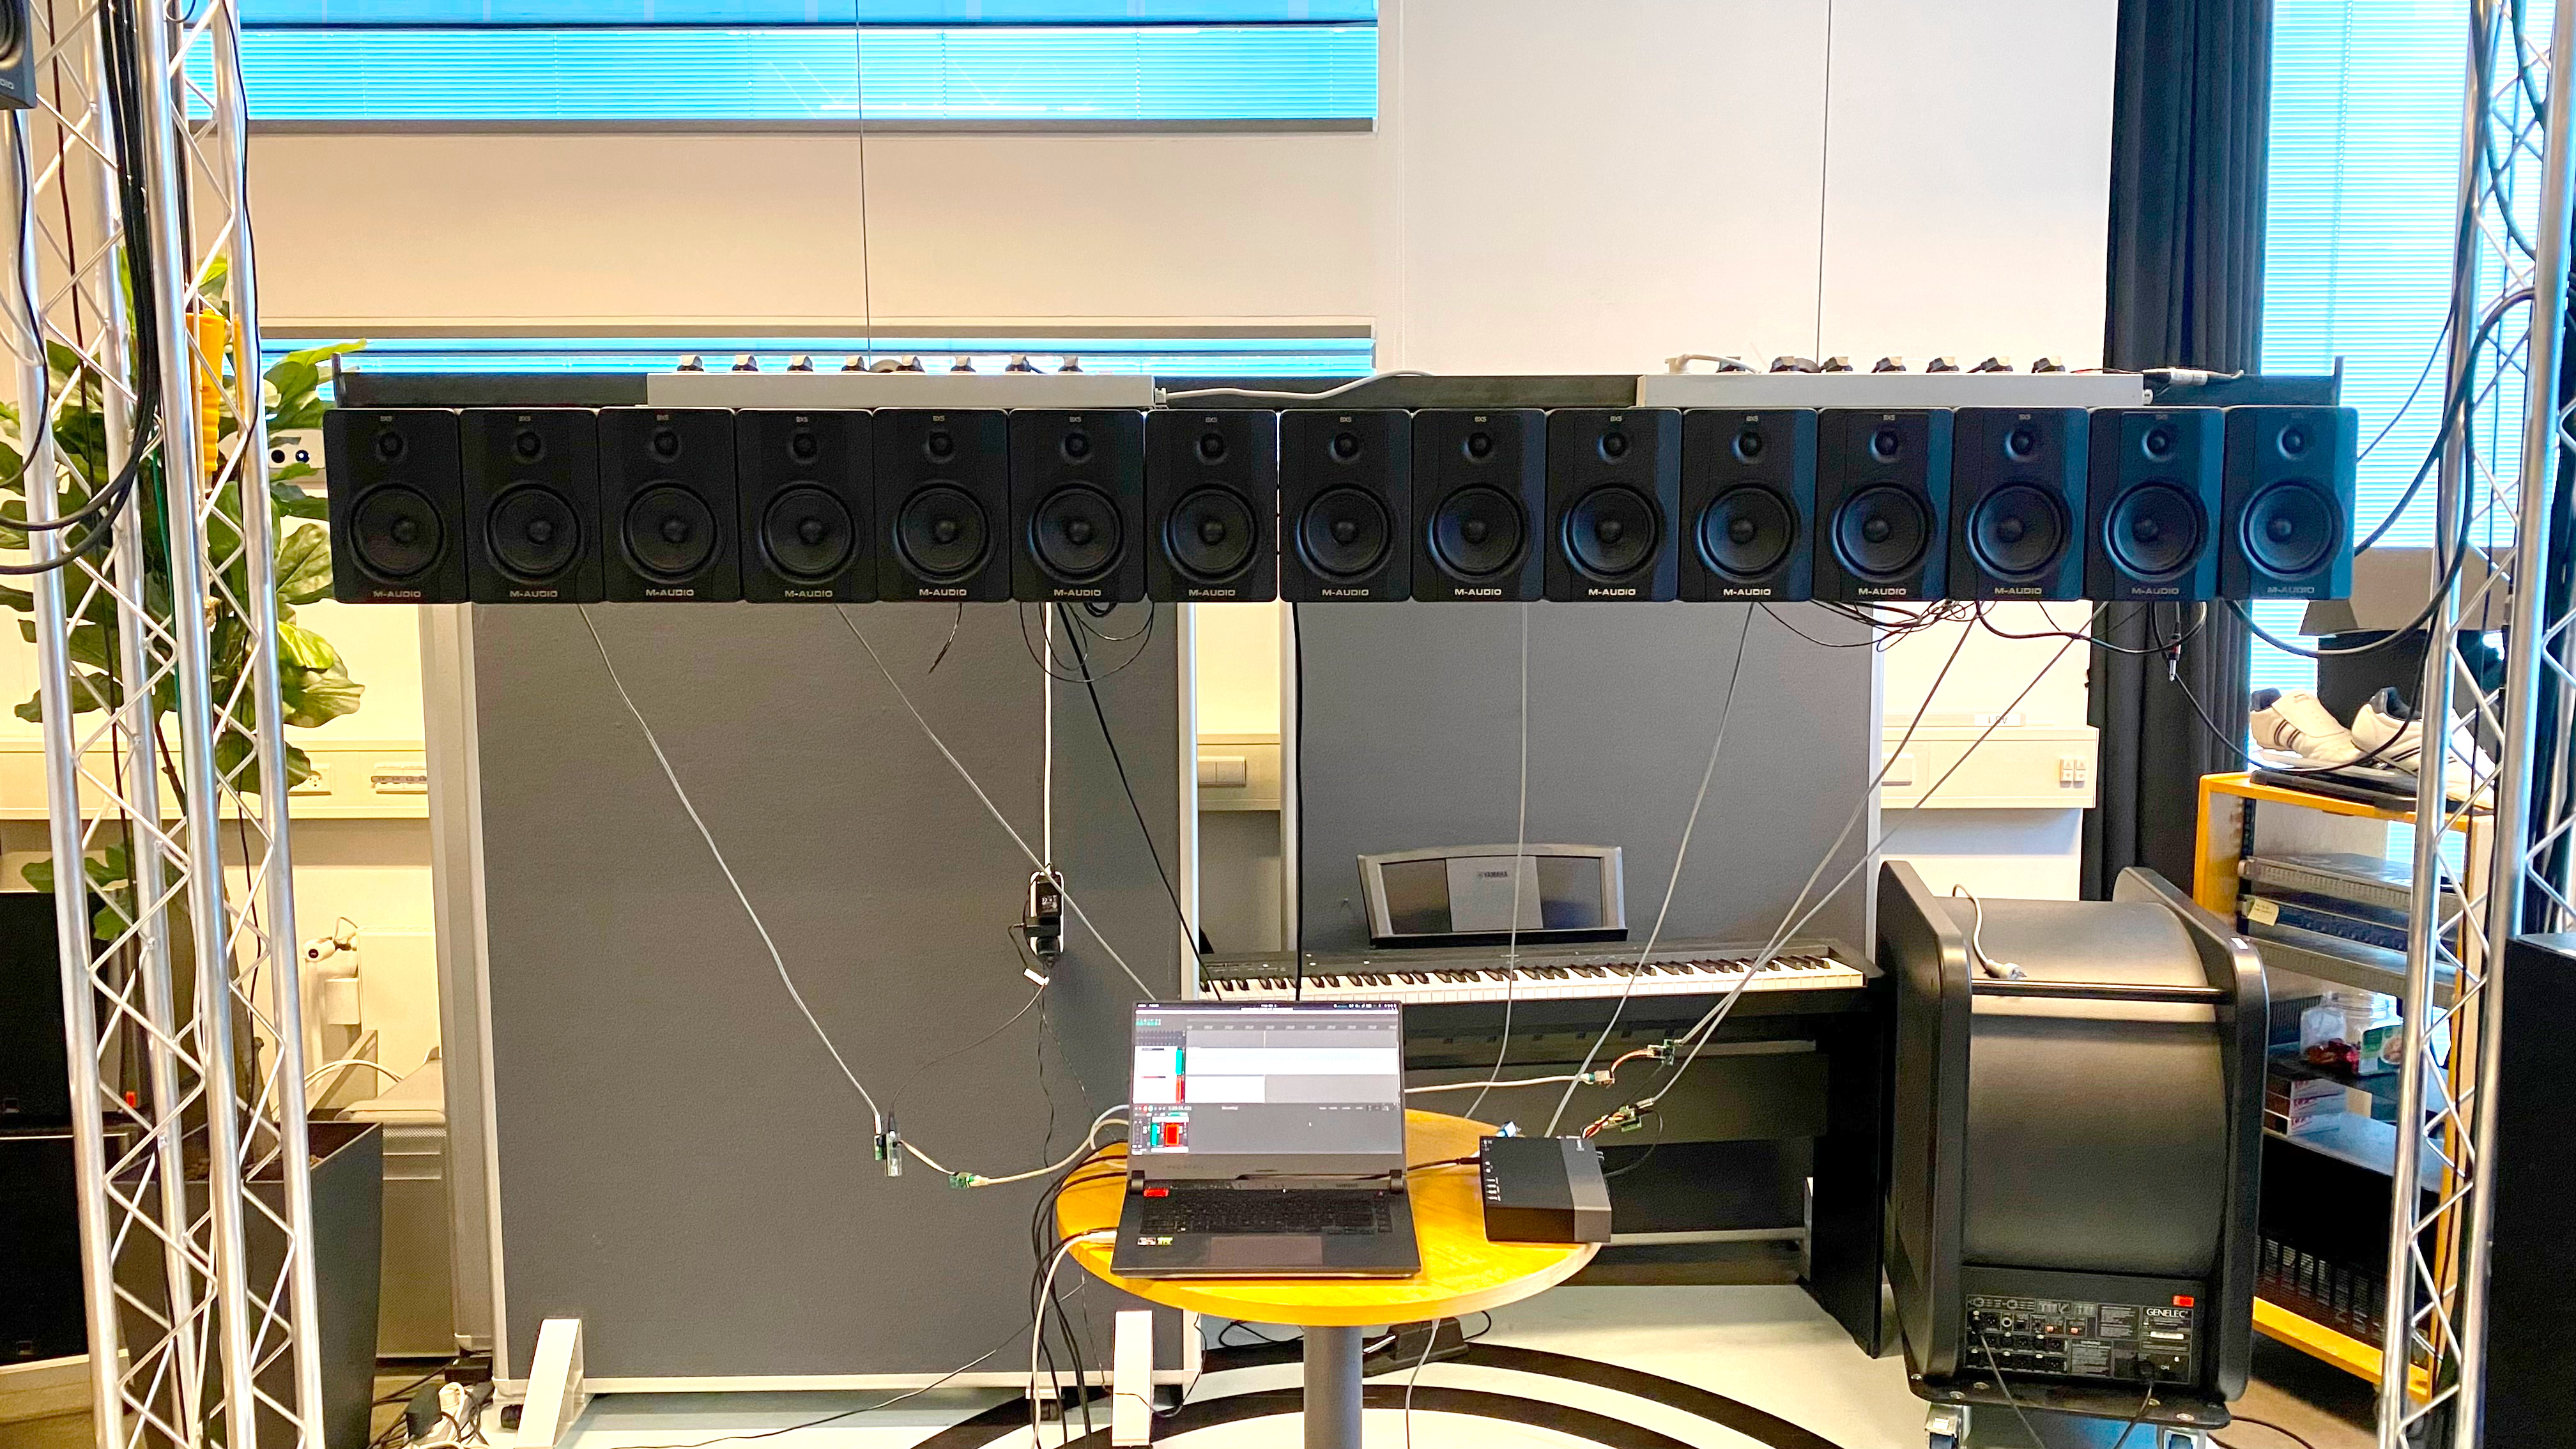
\includegraphics[width=\textwidth]{figures/eval-setup}
    \caption{
        System configuration for technical and perceptual evaluation.
        Eight hardware modules connected to fifteen loudspeakers \textemdash{}
        seven of the modules produced output for two loudspeakers each; the
        final module used only its first output channel.
    }
    \label{fig:eval-setup}
\end{figure}

Possessing technical underpinnings, but ultimately being designed to
serve immersive auditory ends, it was important to consider the performance of
the system described and developed in \secref{sec:method} in terms of
both its technical capabilities and the quality of the perceptual effects it
was able to support.
The success of the system as platform for audio spatialisation techniques is
contingent on it being composed of effective solutions to the challenges posed
by distributing audio processing across a local area network.
It is of limited worth, however, as a technical exercise in isolation;
the subjective assessment provided by listeners may help identify the most
critical aspects of the technical implementation and guide future development.

\subsection{Technical Evaluation}\label{subsec:technical-evaluation}

\begin{figure}[ht]
    \centering
    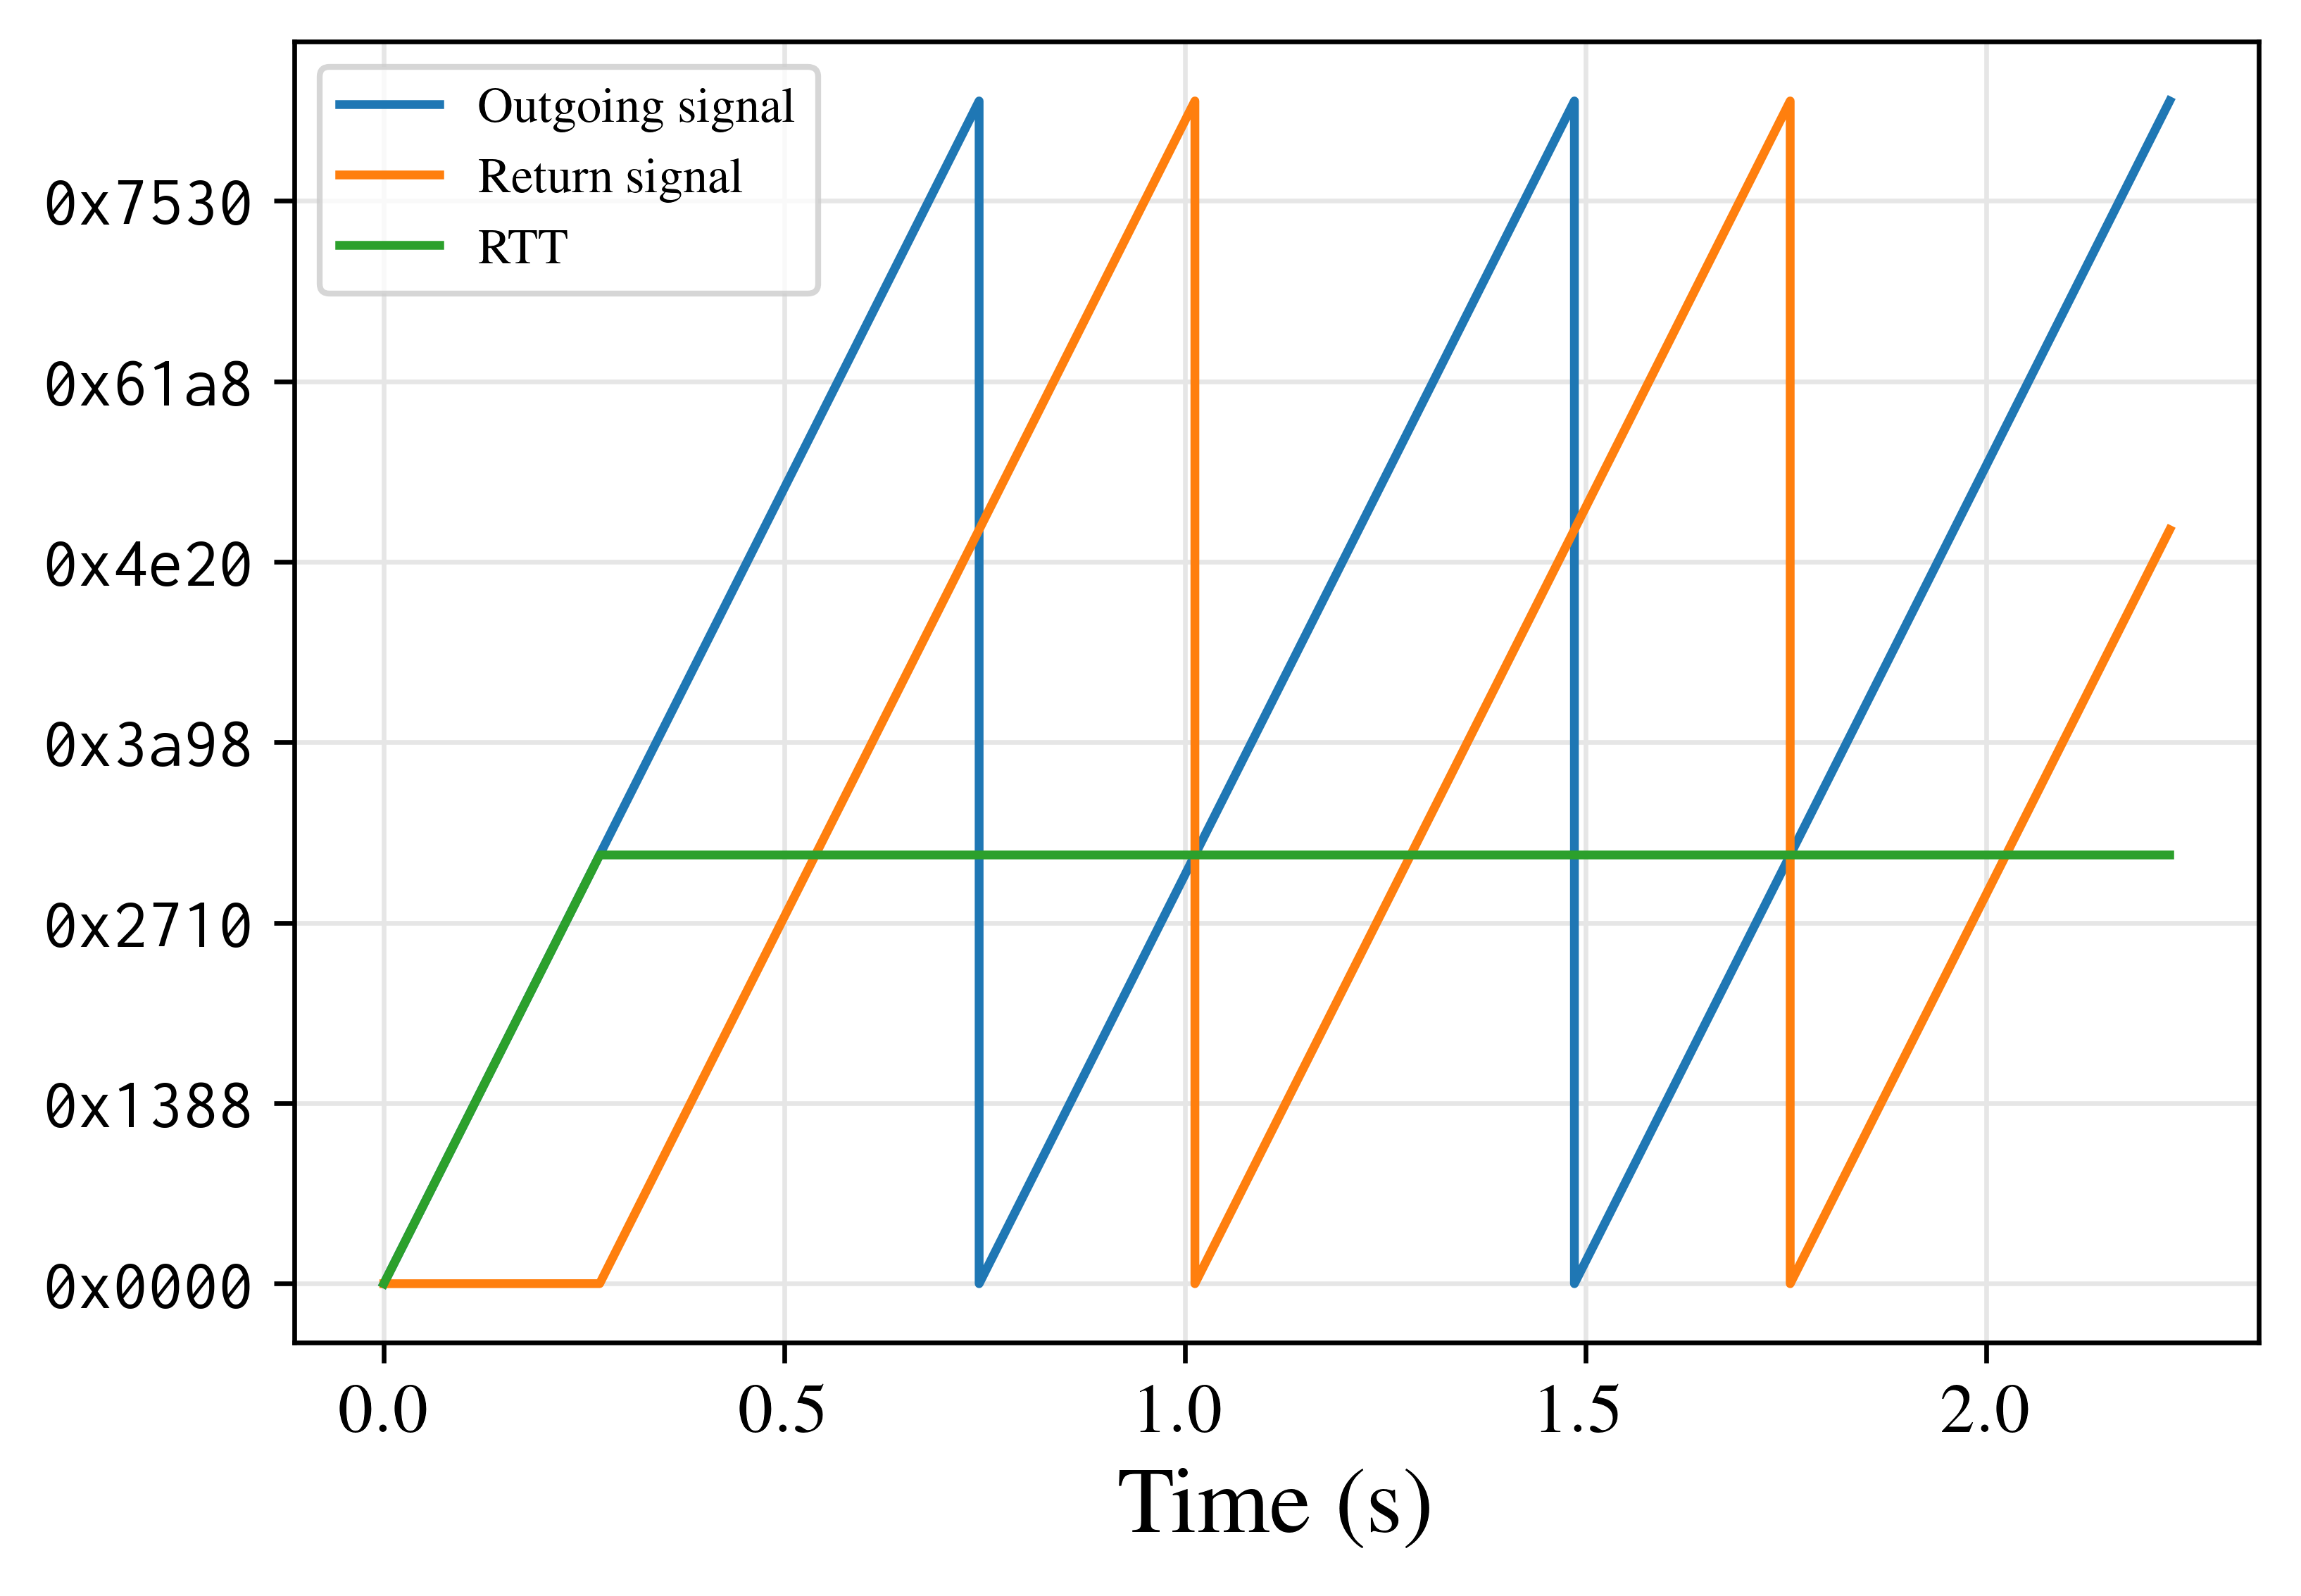
\includegraphics[width=.5\textwidth]{figures/test-signal}
    \caption{
        Illustration of the use of a test signal, a unipolar sawtooth wave,
        to measure round trip time.
        Subtracting the return signal from the outgoing signal gives the time
        (in samples) between transmission and reception.
    }
    \label{fig:test-signal}
\end{figure}
\noindent
Of most pressing technical concern is the matter of synchronicity between the
hardware modules.
To assess this, a similar approach was taken to that found
in~\citep{rushton_microcontroller-based_2023}
and~\citep{gabrielli_networked_2012}.

\subsubsection{Round Trip Time}
To measure transmission round trip time (RTT), the server transmitted a unipolar
sawtooth wave of unit amplitude increment to the multicast group, and each
client, upon receiving the signal simply returned it immediately to the group to
be consumed by the server.
At the server side, the return signal, $x_{\text{ret}}$, was subtracted from the
outgoing signal, $x_{\text{out}}$, at the time of reception, with round trip
time found as:
\begin{equation}
    \label{eq:rtt}
    \text{RTT} = \begin{cases}
                     x_{\text{out}} + \max_{\text{int16}} - x_{\text{ret}}, &x_{\text{out}} < x_{\text{ret}}, \\
                     x_{\text{out}} - x_{\text{ret}}, &\text{otherwise},
    \end{cases}
\end{equation}
where $\max_{\text{int16}}$ is the maximum value representable by a
signed 16-bit integer, \texttt{0x7fff} (\numDec{32767}).

The resulting value is the number of samples elapsed between transmission and
reception (see \figref{fig:test-signal}).
Since there is one source of transmission, for multiple clients, comparing RTT
offers a means to assess inter-client synchronicity.
Server-to-client latency cannot be measured in this way, but that can be
inferred to be around half of, and, of course, certainly not greater than, the
RTT.\

\subsubsection{Clock Drift/Skew}
A unipolar sawtooth wave of unit amplitude increment was generated on the
clients, subtracted from the incoming sawtooth wave from the server, and the
difference (found as per equation~\eqref{eq:rtt}) returned to the multicast
group for consumption by the server.
Under ideal conditions, the incoming signal and the one being generated on a
given client, while almost certainly not synchronised, should be out of phase by
some constant value;
if this value changes then relative drift has occurred between server and
client.
%While not of direct relevance to synchronicity,
The client-side clock-adjustment strategy was designed to minimise the reliance
on the adaptive resampling approach that it complements;
low drift would be indicative of the effectiveness of that strategy.

\begin{figure}[ht]
    \centering
    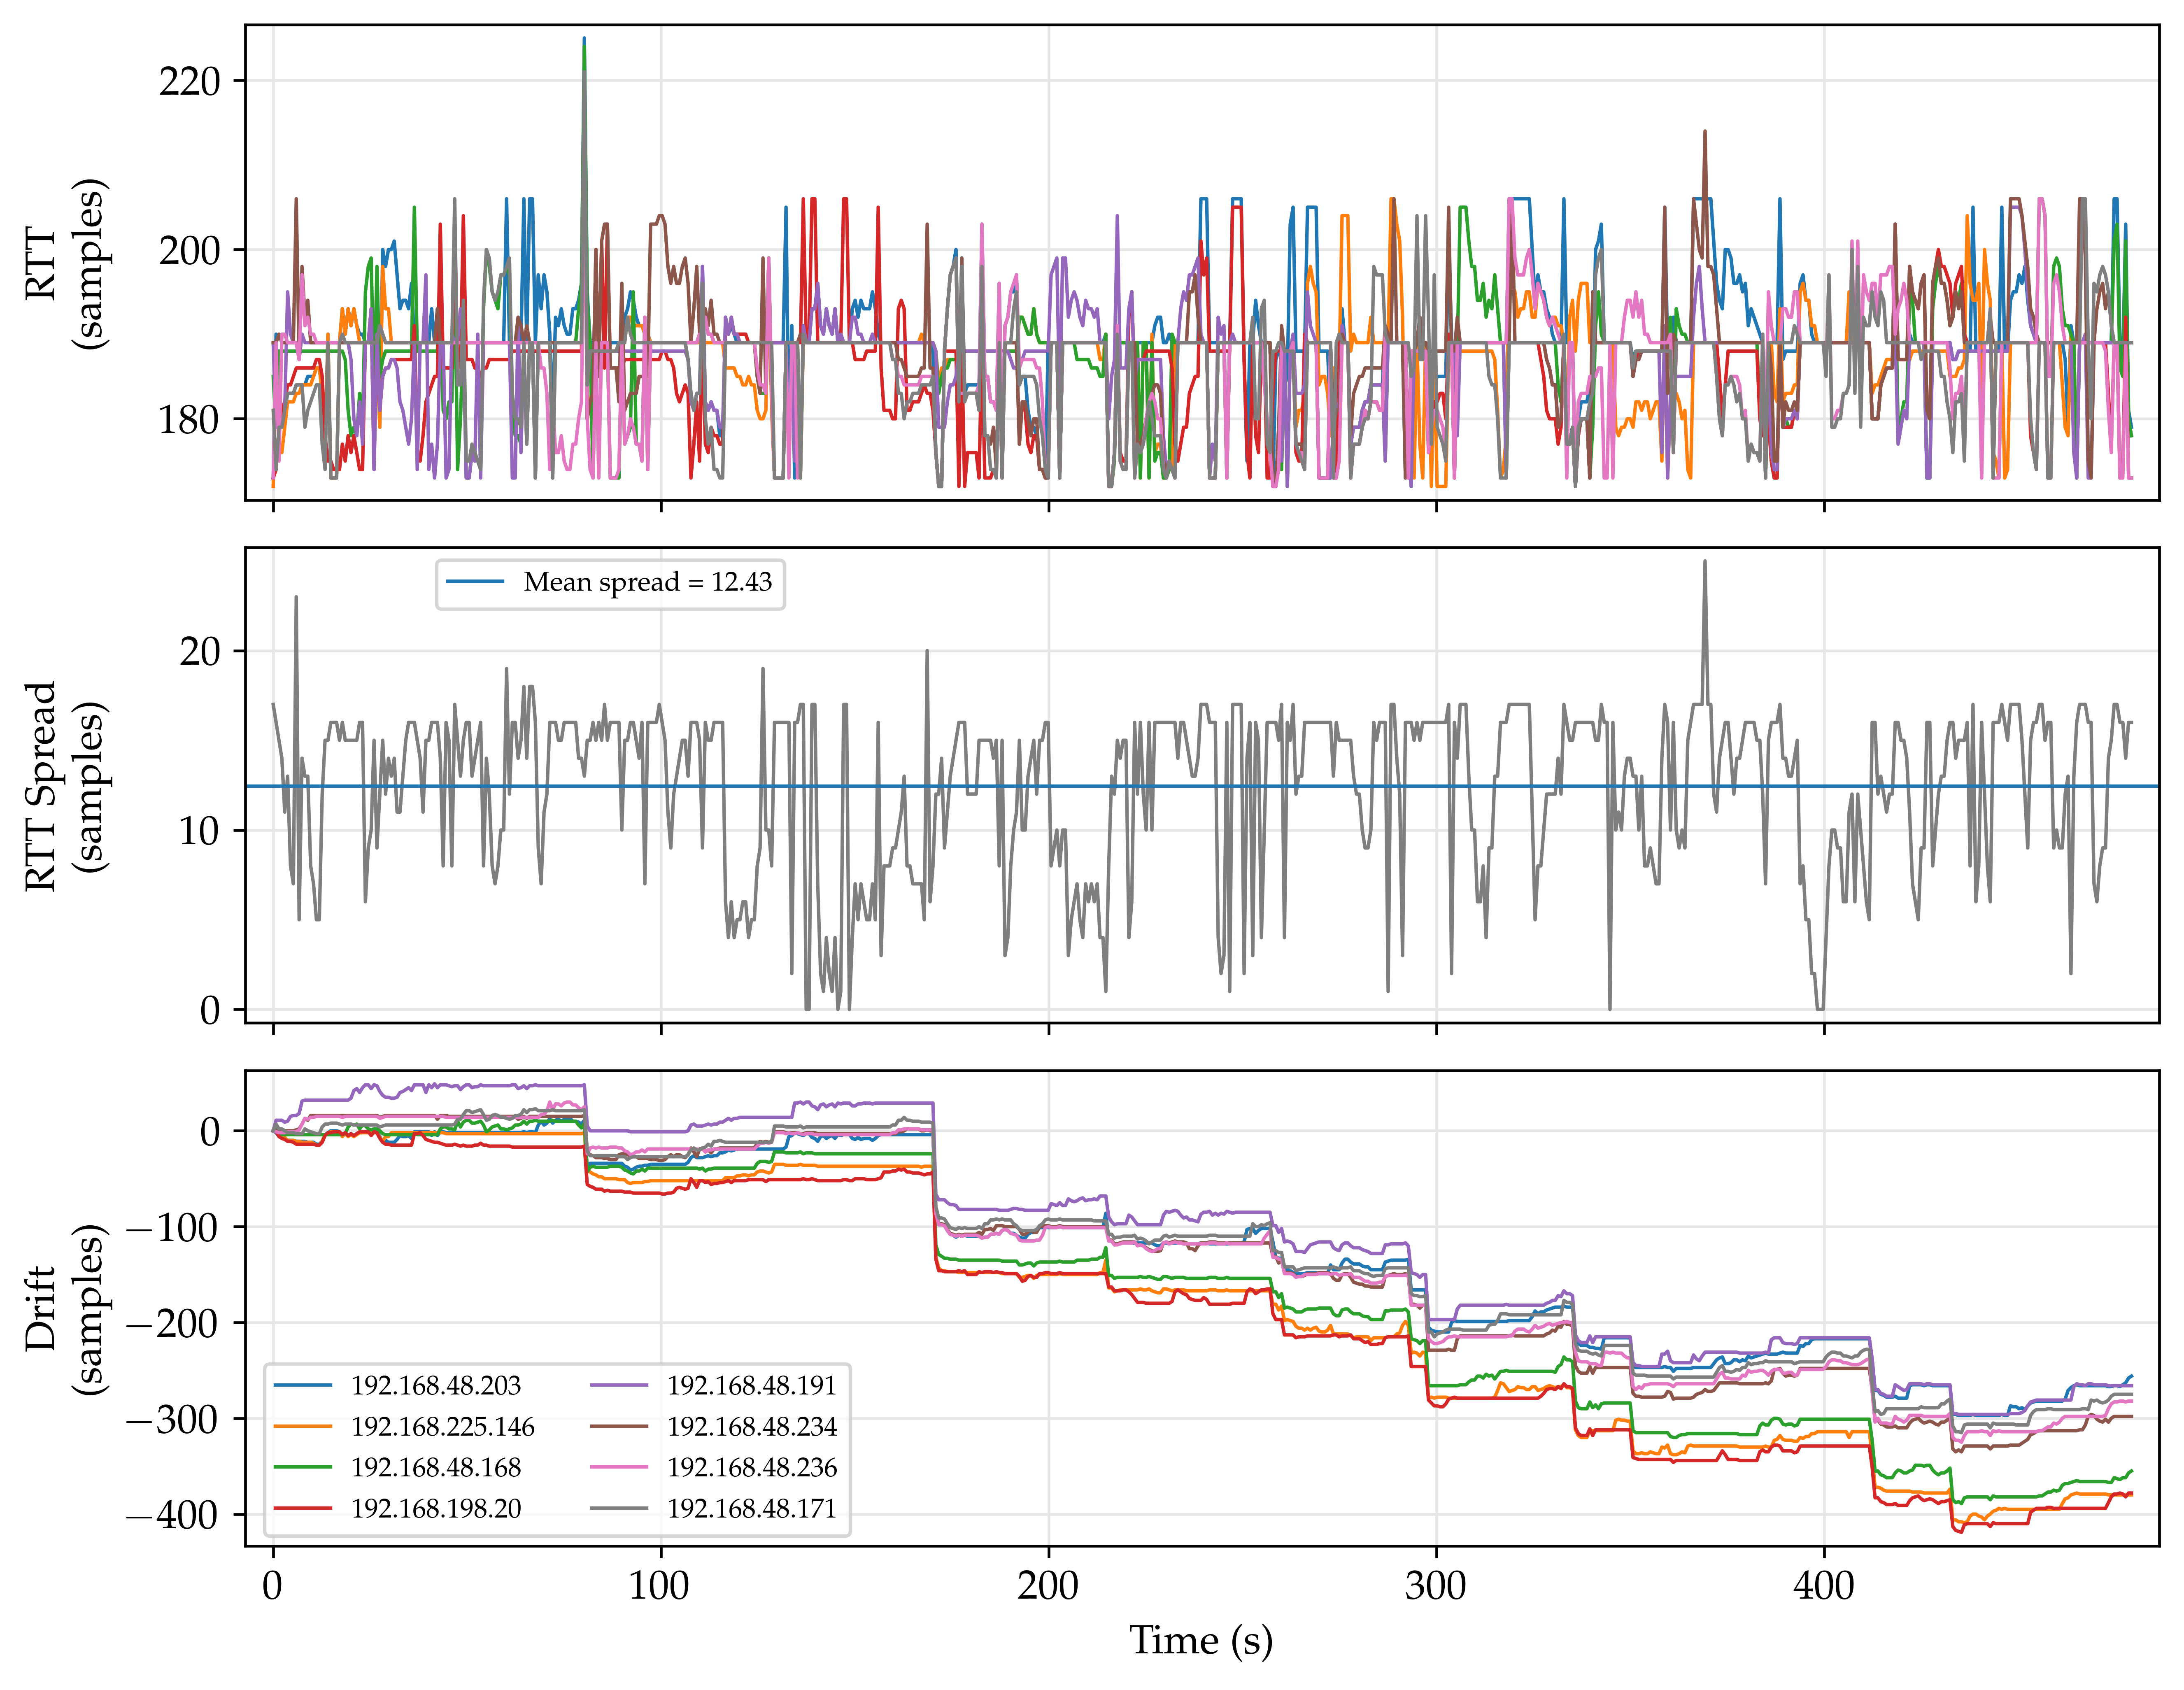
\includegraphics[width=\textwidth]{figures/rtt_drift_16}
    \caption{
        Round-trip time, RTT spread, and clock drift measurements for eight
        networked audio clients, for a networked audio session of eight minutes'
        duration.
        Audio buffer size, 16 samples, sampling rate \qty{44.1}{\kHz}.
        The legend in the bottommost plot applies also to the upper plot.
        Round-trip time, in samples, measured at the server, and found as the
        difference between an outgoing sawtooth wave and its returning
        counterparts from each of eight connected clients.
        Round-trip time spread found as the range ($\text{RTT}_{\max} -
        \text{RTT}_{\min}$), in samples, at each point in time, of
        round-trip times reported for all eight clients.
        Mean spread is the arithmetic mean of RTT spread values taken across
        the entire test.
        Drift, in samples, found as the difference between an outgoing sawtooth
        wave and a sawtooth wave generated on each client, that difference
        returned to the multicast group for consumption by the server.
    }
    \label{fig:rtt-drift-16}
\end{figure}

Initial RTT and relative drift measurements for eight clients are shown in
\figref{fig:rtt-drift-16}.
Mean RTT spread, describing the average temporal interval over which clients
were distributed over the course of the test, is promising, the 12.43 sample
interval corresponding with approximately \qty{282}{\us}.
RTT is clustered around a respectable 190 samples ($\sim$\qty{4.3}{\ms}).

That visual clustering, coupled with the apparent tendency for RTT spread to
lie at around 16 samples (i.e.\ precisely one buffer), suggest, however, a
certain over-aggressiveness in the resampling strategy, perhaps resulting in a
polarisation of clients to the temporal extremes of the interval between their
audio interrupts.
What \figref{fig:rtt-drift-16} does not show, and, given the short timescales
involved, is not easily represented in such a diagram, is the rate of relative
inter-client movement, i.e.\ the rate of change of asynchronicity.
Cursory, subjective assessment of the system's audible output revealed that,
given the rapid rate of relative movement between clients, in this state it
would not stand up to perceptual testing.

Transmitting a signal consisting of white Gaussian noise to the clients and
delivering this to their audio outputs without further processing \textemdash{}
seeking, essentially, to sonify QoS \textemdash{} an aggressive phasing, or
time-varying comb-filter effect was clearly audible.
This effect is visualised in \figref{fig:spectrograms}(A); ideally (and
subject to the frequency of the response of the microphone used) an ambient
recording of a white noise source would correspond with a magnitude spectrogram
exhibiting equal intensity across the frequency range at all times; clearly,
though, there are regions of greater and lesser intensity, and these regions
shift and change rapidly over time.
In addition to the above, tests involving the reproduction of signals
containing steady-state harmonic content revealed obtrusive audible artefacts.

\begin{figure}[ht]
    \centering
    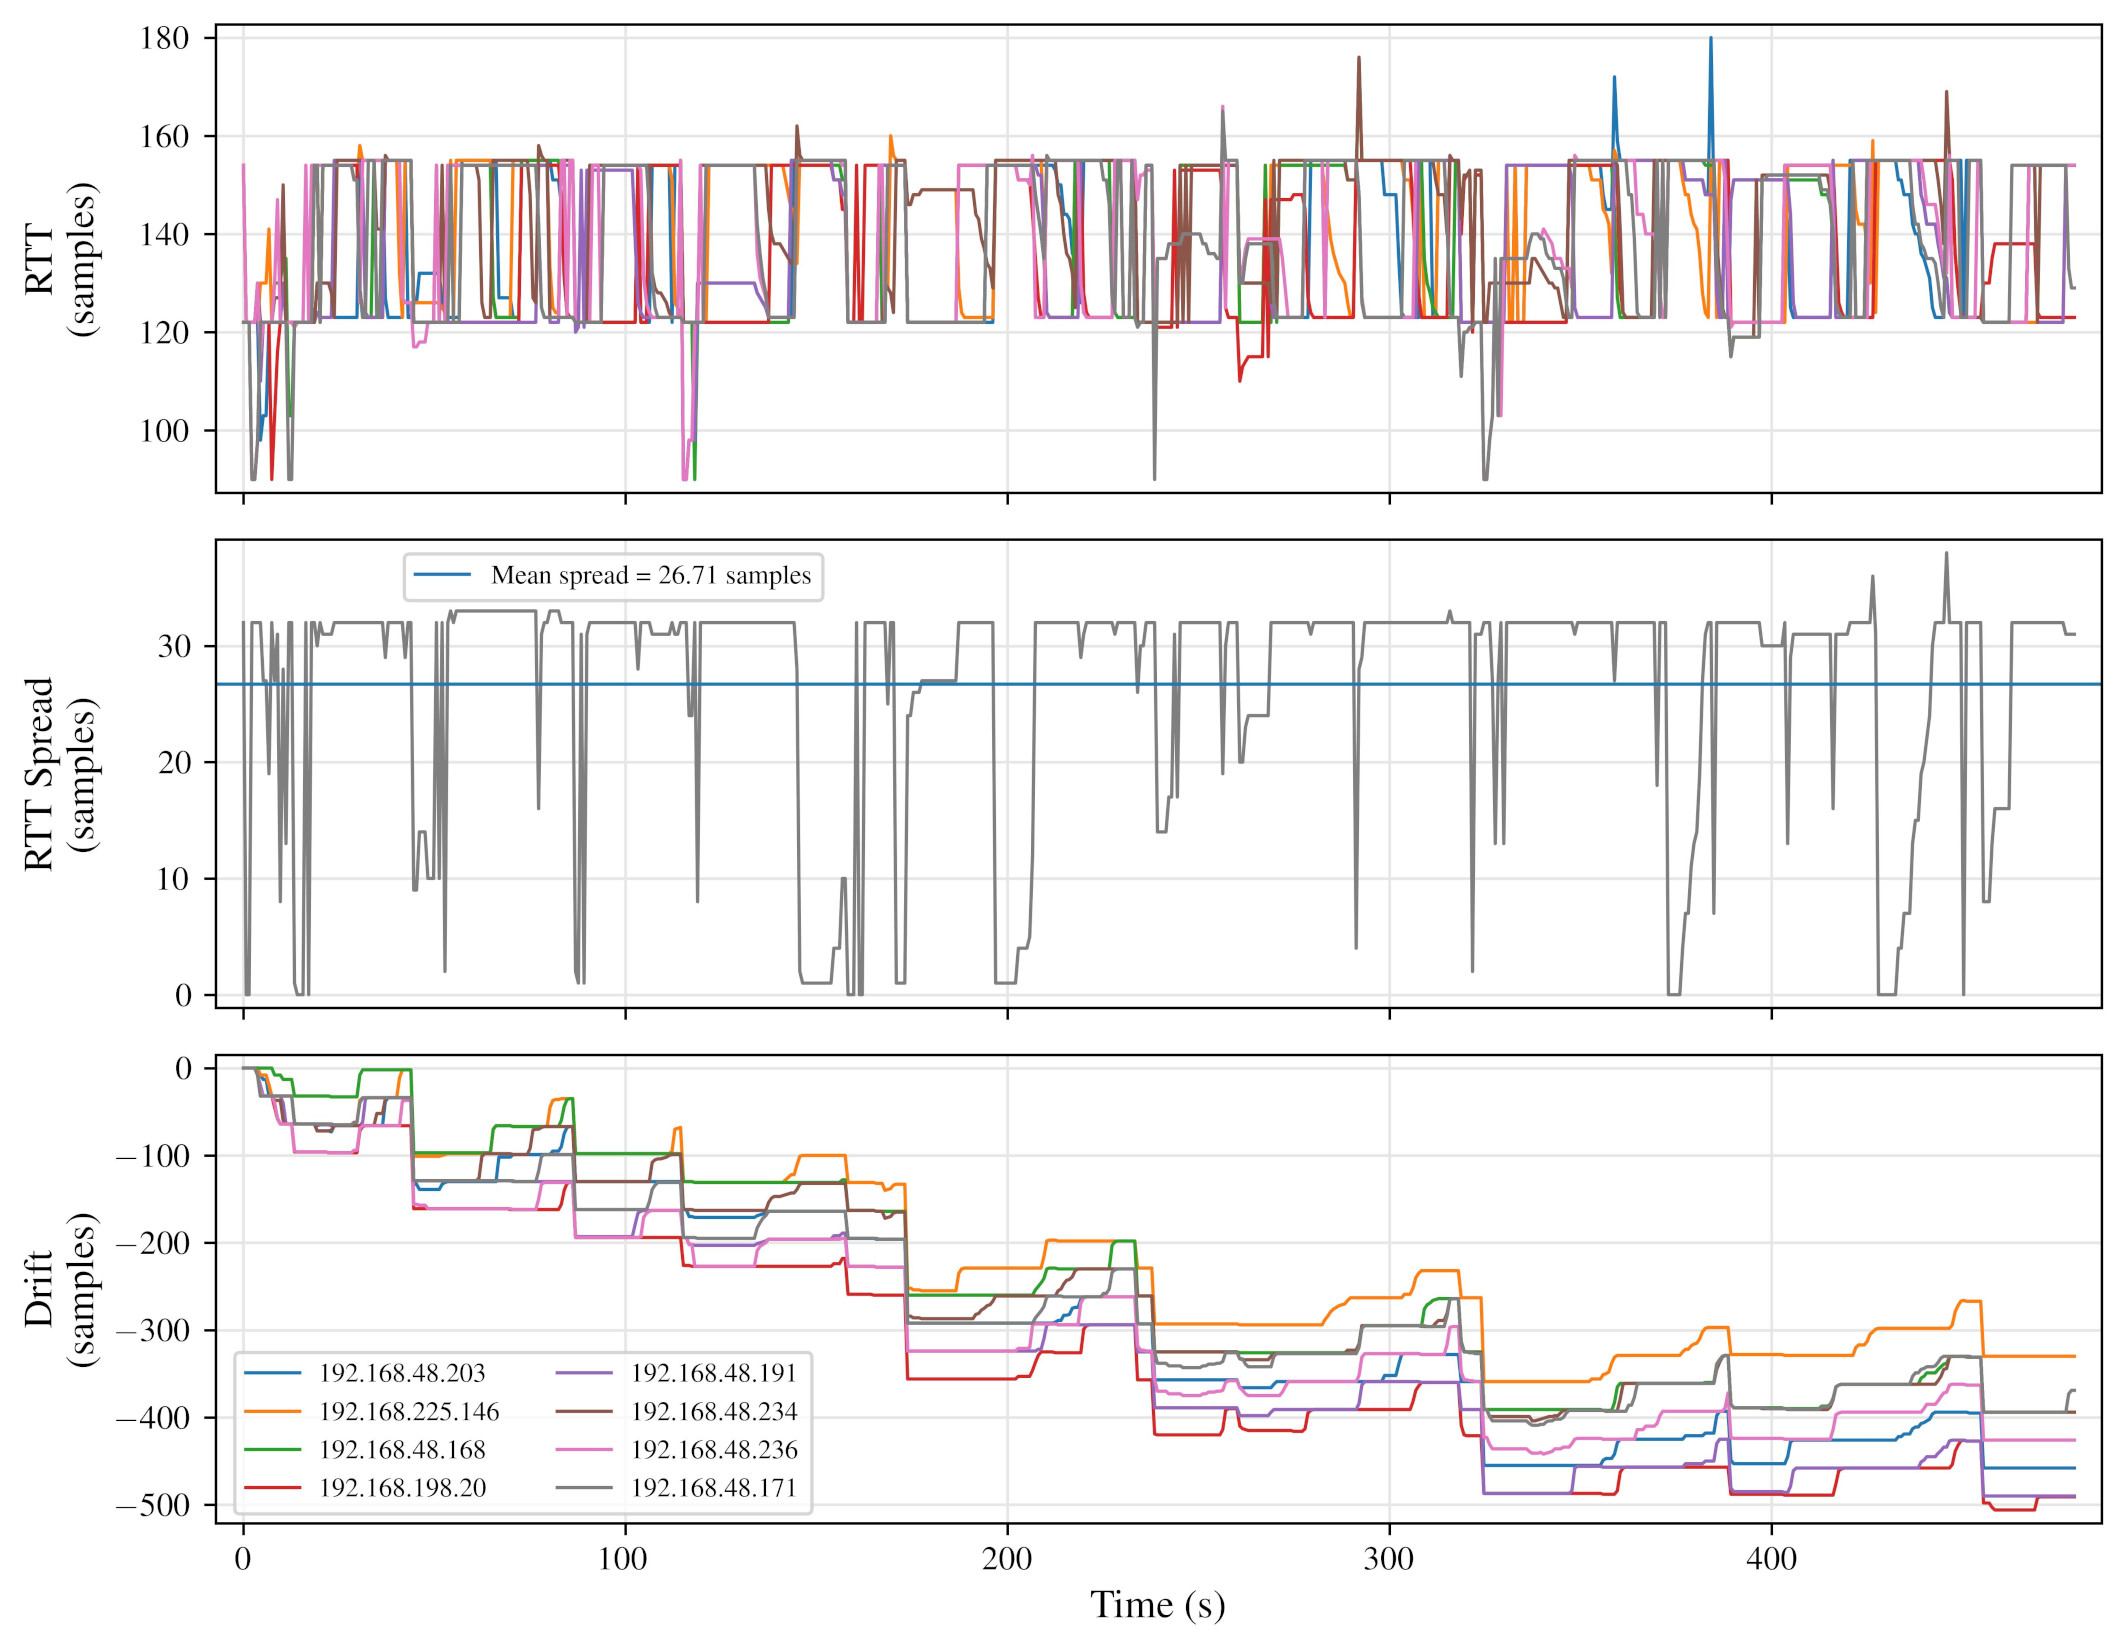
\includegraphics[width=\textwidth]{figures/rtt_drift_32}
    \caption{
        Round-trip time, RTT spread, and clock drift measurements
        for eight networked audio clients, for a networked audio session of
        eight minutes' duration.
        Audio buffer size, 32 samples.
    }
    \label{fig:rtt-drift-32}
\end{figure}

A buffer size of 16 samples had been selected in an attempt to minimise the
duration of the window of inter-client synchronicity, and to maximise the
number of channels that could be transmitted over the network, subject to
restrictions posed by the MTU (see
\secref{subsubsec:transmission-considerations}).
Recalling, however, that previous
work~\citep{rushton_microcontroller-based_2023}
had employed a 32-sample audio buffer, equivalent measurements were taken for
the larger buffer size, the results of which are depicted in
\figref{fig:rtt-drift-32} and \figref{fig:spectrograms}(B).

\begin{figure}[ht]
    \centering
    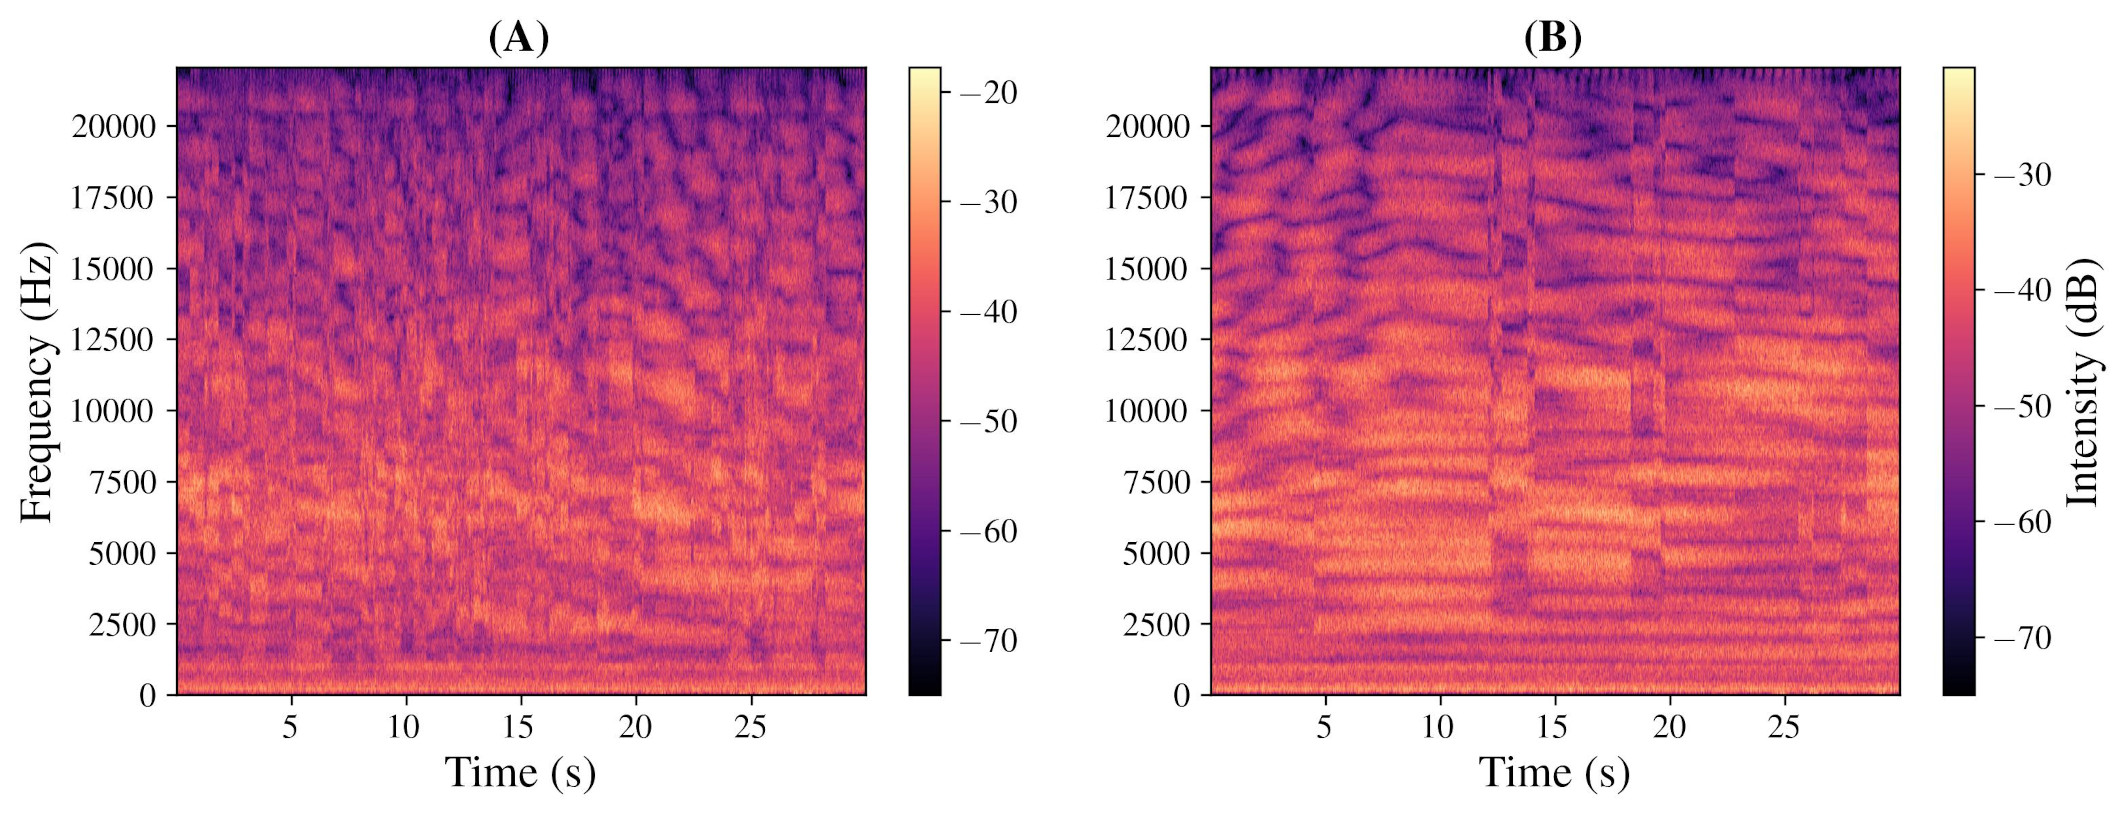
\includegraphics[width=\textwidth]{figures/wgn_specgram_16_32}
    \caption{
        Magnitude spectrograms of ambient, monophonic recordings of a
        reproduction of white Gaussian noise by a group of eight networked
        audio clients driving an array of fifteen loudspeakers spaced at
        intervals of \qty{.175}{\m}.
        Capacitor microphone placed $\sim$\qty{2}{\m} from the
        speaker array.
        Audio buffer (and thus network packet) size (A) 16 samples;
        (B) 32 samples.
    }
    \label{fig:spectrograms}
\end{figure}

Again, visually, there is an apparent clustering in the RTT recordings, with
clients spending large periods separated by around one buffer's worth of
samples ($\sim$\qty{726}{\us}), seemingly often grouped at either
extreme of the interval of one audio buffer.
The mean RTT spread, $\sim$\qty{626}{\us}, is comparable with results
from prior work, but, disappointingly, slightly less favourable.
Importantly, however, and as demonstrated in \figref{fig:spectrograms}(B), the
rate of relative inter-client temporal movement was much improved by the switch
to a 32-sample buffer.
Although exhibiting similar visual striations to the spectrogram for the test
at 16 samples, fluctuations occur less frequently, and seemingly more
gradually.
Indeed, subjectively-speaking, the disruption caused by the phasing effect
that afflicted the 16-sample buffer implementation was significantly reduced,
as was the presence of audible artefacts affecting harmonic signals.
Thus it was the version of the system employing a buffer size of 32 samples
that was exposed to perceptual evaluation.

Clock drift measurements in \figsref{fig:rtt-drift-16}{fig:rtt-drift-32} exhibit
comparable trends.
Increasing negative drift over time is indicative of the clients running faster
than the server.
Visually, there is evidence that client clocks adjust to approximate parity
with the server for periods of time, perhaps falling slightly slower (e.g.\
the drift plot in \figref{fig:rtt-drift-16}, between 100 and 160 seconds), but
periodically demonstrate large negative steps.
These leaps are far from desirable, and suggestive of there being significant
room for improvement in the devised strategy for PLL adjustment.

\subsubsection{Discussion}\label{subsubsec:discussion-tech}

The temporal clustering and polarisation seen in
\figsref{fig:rtt-drift-16}{fig:rtt-drift-32} is indicative of two points for
concern with regard to technical implementation:
the read-write difference threshold strategy may be insufficiently forgiving,
forcing the read position into deleteriously fluctuating increment changes in
response to periods of jitter.
And without a master clock to indicate to each client the beginning of each
output audio block, even with clock rates perfectly aligned, there is nothing
to guarantee agreement of the timing of audio interrupts at the client side.

To avoid sudden, large or `unrealistic' clock adjustments, clients assess
the drift ratio as assessed via the ratio of network packet
transmission to reception and, if it lies beyond an arbitrary threshold,
simply resets the clock to the default \qty{44.1}{\kHz}.
Resets of this sort may account for the large steps seen in the drift plots
in \figsref{fig:rtt-drift-16}{fig:rtt-drift-32}.
It is clear that this strategy could be significantly improved upon.

\subsection{Perceptual Evaluation}\label{subsec:perceptual-evaluation}

The WFS system was subjected to an informal perceptual evaluation, in which
participants were presented with a virtual sound source at various locations
and asked to indicate, on a diagram of the virtual sound field, the point
at which they estimated the sound had emanated from.
The informality of the experiment arose in part as a consequence of the
listening environment not being acoustically treated, and there being sources
of ambient sound in the laboratory in which the WFS system was installed.
Furthermore, the speaker array (\figref{fig:eval-setup}) consisting of fifteen
speakers, but each hardware module producing two audio output channels,
the second channel of the right-most module was not used;
for eight modules, however, the WFS plugin assumed a virtual sound field
spanning sixteen speakers, thus it was possible to position a virtual sound
source horizontally beyond the rightmost extent of the speaker array.
Ultimately the aim of the experiment was to draw some preliminary, guiding
conclusions as to the effectiveness of the distributed WFS system in
triggering listeners' localisation cues, its technical and installation
shortcomings notwithstanding.

In terms of the design of the auditory stimulus, it was felt that listeners
would be most comfortable localising a naturalistic sound.
Rather than use blasts white noise as in~\citep[ch.~6]{verheijen_sound_1998},
but wishing to minimise the potential effects of frequency-dependent
localisation interference due to spatial aliasing, a broadband stimulus
was selected in the form of a close-mic recording of a snare drum.
The recorded sample was repeated three times in succession at intervals of
\qty{.125}{\s}, and, again in the interests of adding a natural quality to the
sound, with slight variations in amplitude (the second iteration of the sample
was played marginally quieter than the first; the third slightly louder).

Participants were given a brief description of the system under evaluation,
and informed that they should expect to hear sounds that appeared to emanate
from `behind' the speaker array, from which they stood at a distance of
$\sim$\qty{2}{\m}.
Eight different virtual source positions were specified via automation of the
$x$ (lateral) and $y$ (longitudinal distance) components of the position of a
node in the WFS plugin interface.
The range of the $x$ component corresponded with the distance from the centre of
the driver of the leftmost speaker to that of the missing sixteenth loudspeaker;
drivers lay at intervals of \qty{.175}{\m}, giving a horizontal axis spanning
\qty{2.625}{\m}.
Longitudinal position was mapped to a range from \qty{0}{\m} (i.e. lying
directly on the speaker array) to \qty{10}{\m} `behind' the array.

For each position, the auditory stimulus was sounded, and repeated at the
participant's request.
Details of the source positions for each test, and the responses given by
eight participants, are displayed in \figref{fig:perceptual}.

\begin{figure}[h!]
    \centering
    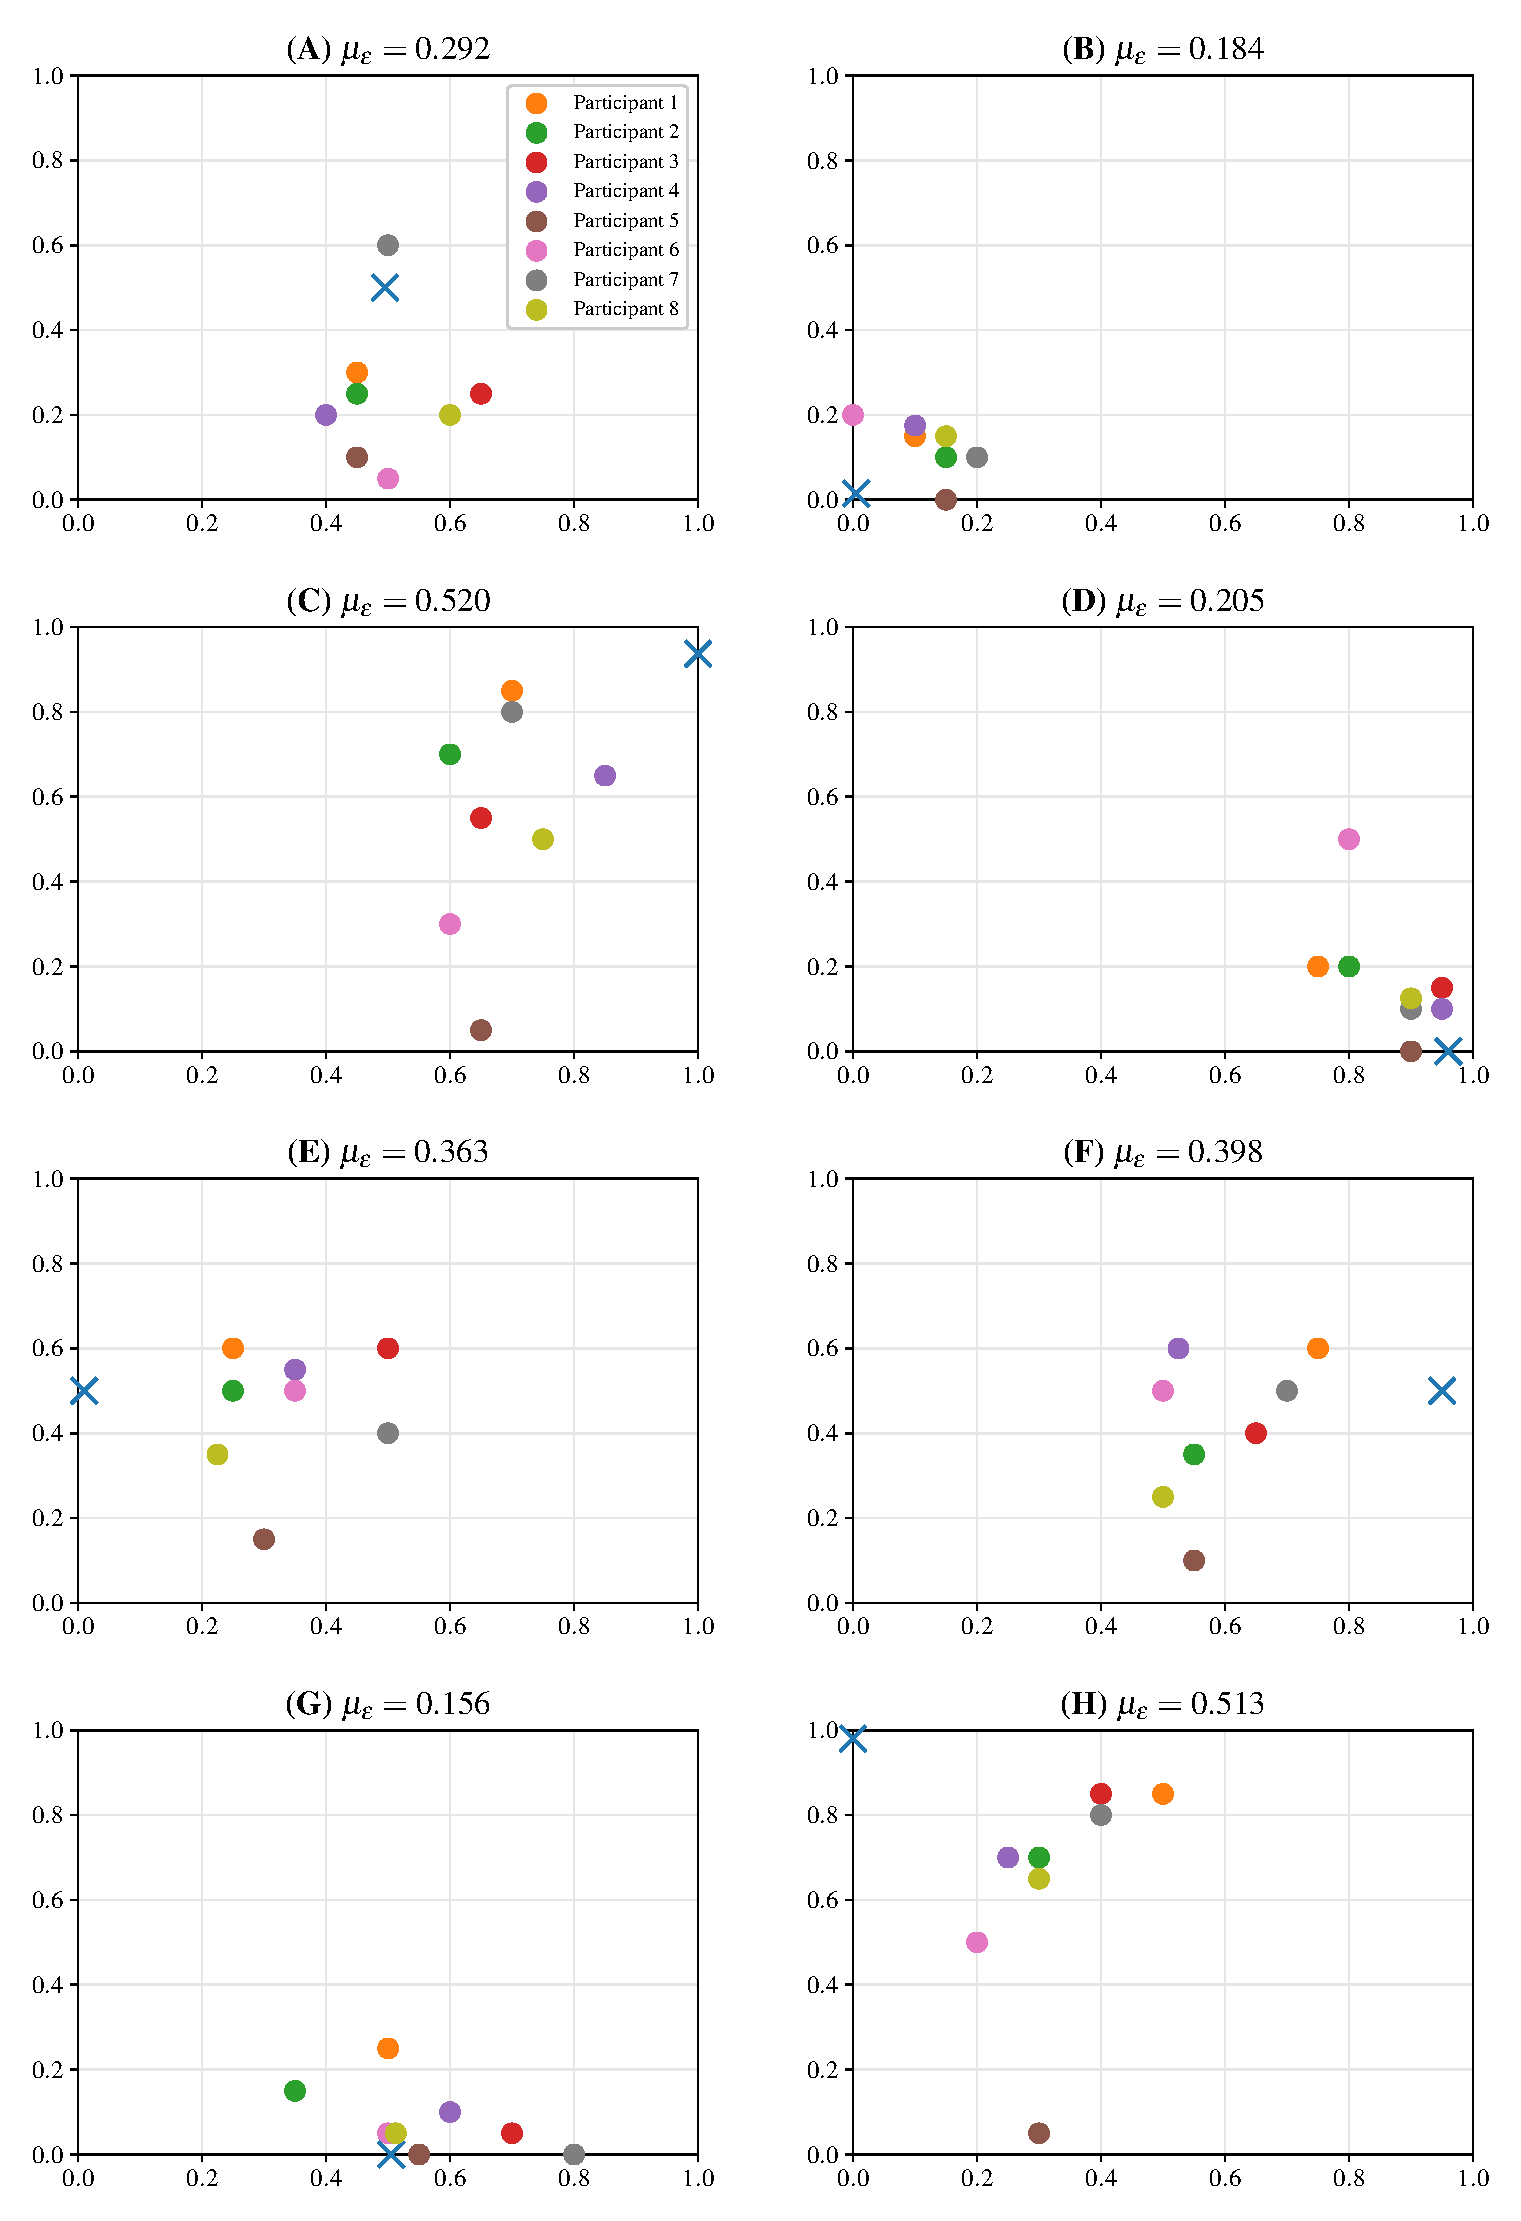
\includegraphics[width=.775\textwidth]{figures/subjective}
    \caption{
        Results of perceptual evaluation of the proposed system.
        Lateral (horizontal axis) and longitudinal (vertical axis) components
        are normalised to $[0, 1]$.
        For each plot, the horizontal axis (i.e. longitudinal component
        equalling 0) corresponds with the location of the speaker array.
        Each plot shows the intended position of the virtual sound source as
        specified by parameters to the WFS plugin interface (cross) and
        estimated sound source positions as reported by participants (dots).
        Each plot is labelled with the mean Euclidean error $\mu_\epsilon$
        between intended position and reported positions.
        Legend in plot \textbf{(A)} applies to all plots.
    }
    \label{fig:perceptual}
\end{figure}

As can be seen, although far from perfect, and with some significant
outliers (e.g.\ the position reported by the fifth participant for test
\textbf{(D)}), certain trends do appear to emerge from the results.
Firstly, responses loosely track the intended positions, with reported
positions most closely corresponding with intended ones for virtual source
locations lying close to the speaker array.
Indeed, tests \textbf{(B)}, \textbf{(D)}, and \textbf{(G)} exhibit the lowest
mean error values between the intended and reported positions.
The results for tests \textbf{(C)} and \textbf{(H)}, exhibit the greatest mean
error, and ambiguity regarding the lateral position of distant sound sources is
perhaps to be expected;
as the distance of a sound source from the listener increases, $r_k - y_k$
tends towards zero, and thus the ITD (and ILD) also approaches zero;
thus, with increased distance the wavefront produced by a sound source (be it a
real sound source or one synthesised under ideal conditions) approximates more
and more closely a plane wave.
In any case, despite this inherent, physical ambiguity, there is a tendency
in results \textbf{(C)} and \textbf{(H)} toward the lateral location of the most
longitudinally distant intended virtual source positions.
Particularly for test \textbf{(C)}, participants seem to have had greater
difficulty in estimating the depth of the virtual sound field; this may simply
be as a function of their developing a familiarity with that aspect of it over
the course of what was only a brief experiment.

Participants were asked for any anecdotal observations they had, based on their
experience of the experiment.
One participant noted, for the first position in particular, that the amplitude
variations between the snare drum strikes gave the impression of a sound source
that was advancing upon the listening position; for the lack of any visual cue
as to the position of the sound source, this is a reasonable conclusion to draw;
it did not, however, ultimately prevent them from reaching a decision with
regard to their estimate for the position of the sound source.
Another, likely hearing the time-varying comb-filter effect, asked whether the
``phasing'' they were hearing was intentional.
A third, also perceiving a similar phenomenon, suggested that they
felt that the sound sources were moving.
Finally, a participant with prior experience working with WFS systems, remarked
that the distance effect (i.e.\ the WFS prefilter) was perhaps a little extreme,
and not altogether realistic.

\subsubsection{Discussion}\label{subsubsec:discussion-percep}

The phasing effect noted by one participant is a consequence of the approach
taken to combating jitter and keeping the clients close, temporally, together,
and as close to the server as possible.
It is clear that the current approach is, at best, too aggressive to be viable
for high-quality audio output.
Furthermore, an unpitched sound source like a snare drum, though audibly
susceptible to the time-varying comb-filter effect described, masks other
artefacts caused by phenomena such as rapid fluctuations in the clients' buffer
read position increment, and sudden, comparatively large audio clock
adjustments.

The above being said, the perceptual test indicates that the system produces
virtual sound sources that listeners are, at least to some extent, able to
localise.
Further, it achieves this at a significantly lower cost-per-channel than any of
the systems discussed in sections \secref{subsubsec:spatial-sota}, and, speakers
and cables excepted, compares favourably with the OTTOSonics system referred to
in \secref{subsec:distributed-audio-systems}, particularly as channel-count
increases, i.e.\ in terms of cost, it has the potential to scale better.
The most costly component of the system is the computer, but this could be
exchanged for any interested user's personal machine, so long as it is able to
run a DAW and has an ethernet interface.
The Teensy modules, including audio shield, cost around \texteuro{45};
eight-port ethernet switches can be purchased for as little as \texteuro{20-30}.
Assuming a computer costing \texteuro{1500}, at 16 channels we can estimate
around \texteuro{120}/channel, dropping to \texteuro{50}/channel for 64
channels.
